\section{Forward Translations}\label{sec:forward-translation}
An abstract translator class analyzes each node of the parsed tree and delegates them to specialized subtranslators. In this process, an object called \gls*{teo} is built. This \gls*{teo} is needed to rebuild a string representation of the mathematical expression after all nodes of the parsed tree were translated.

The parsed tree generated by the \gls*{pom}-tagger is not a mathematical expression tree. The \gls*{pom} project aims to disambiguate mathematical \LaTeX{} expressions and generates an expression tree. However, in the current state, many expressions cannot be disambiguated yet. In consequence, the \gls*{pom}-tagger generates a raw parsed tree where each token in the \LaTeX{} expression is a node in the tree. We call this parsed tree, the \gls*{pom-pt}.

{\sloppy The overall forward translation process is explained in~\Cref{fig:forward-trans}. All translation patterns and related information are stored in the DLMF/DRMF tables. These tables are converted by the \verb|lexicon-creator| to the \verb|DLMF-macros-lexicon| lexicon file. Together with the \verb|global|-\verb|lexicon| file, the \gls*{pom-pt} will be created by the \gls*{pom}-tagger. The \verb|latex-converter| takes a string representation of a semantic \LaTeX{} expression and uses the \gls*{pom} engine as well as our \verb|Translator| to create an appropriate string representation for a specified \gls*{cas}.}

\begin{figure}[ht]
	\vspace{-10pt}
	\centering
	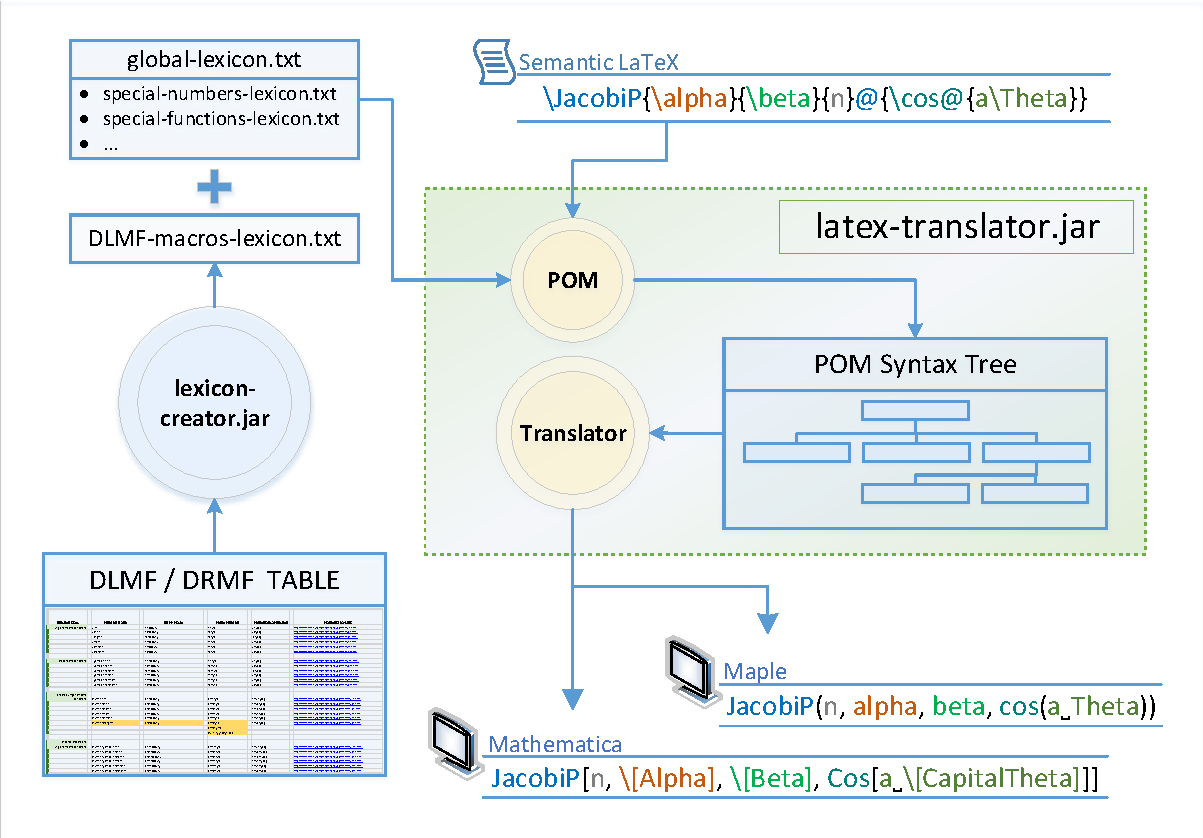
\includegraphics[clip, trim=0.2cm 0.2cm 0.2cm 0.2cm, scale=0.72]{ForwardTranslationProcess.pdf}
	\caption{Process diagram of a forward translation process. The \gls*{pom}-tagger generates the \gls*{pom-pt} based on lexicon and \gls*{json} files. The \gls*{pom-pt} will be translated to different \gls*{cas}.}
	\label{fig:forward-trans}
	\vspace{-10pt}
\end{figure}

\subsection{Analyzing the PoM-Parsed Tree}\label{subsec:analyze-mlp}
Since the \gls*{bnf} does not define rules for semantic macros, each argument of the semantic macro and each $@$ symbol are following siblings of the semantic macro node. That is the reason why we stored the number of parameters, variables and $@$ symbols in the lexicon files. Otherwise, the translator could not find the end of a semantic macro in the \gls*{pom-pt}.

\begin{figure}[ht]
	\centering
	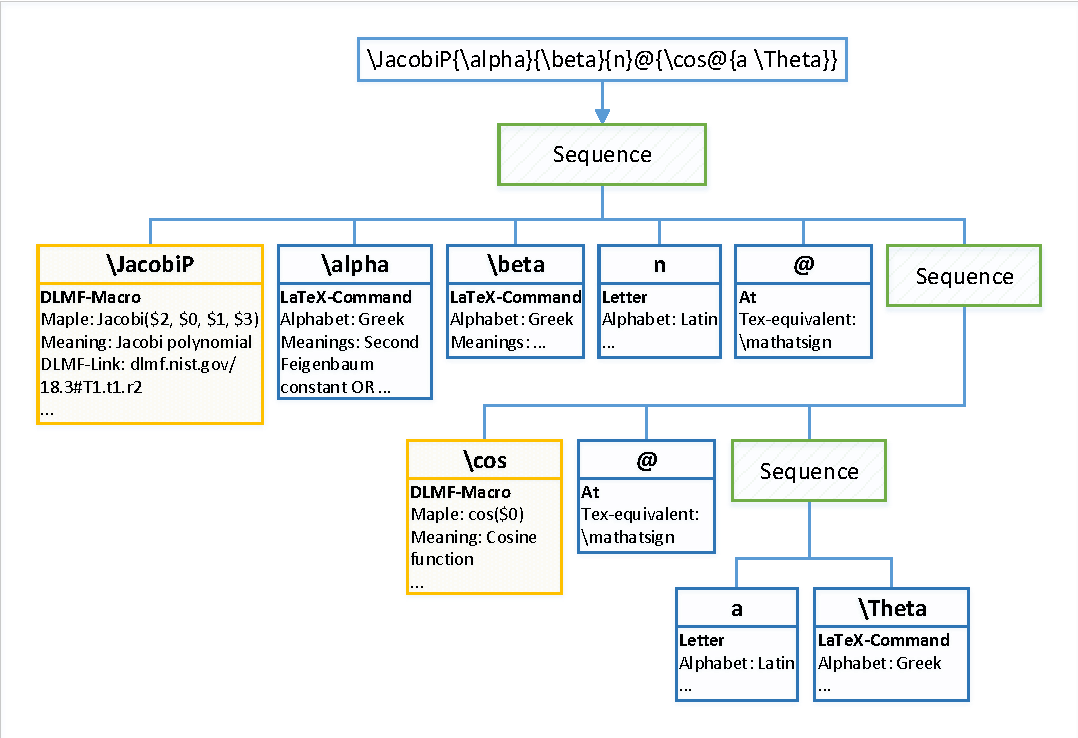
\includegraphics[clip, trim=0.2cm 0.2cm 0.2cm 0.2cm, scale=0.75]{SyntaxTreeUseCase.pdf}
	\caption{pom-pt for a Jacobi polynomial using the DLMF/DRMF \LaTeX{} macro. Each leaf contains information from the lexicon files.}
	\label{fig:syntax-tree-usecase}
	\vspace{-10pt}
\end{figure}

\begin{wrapfigure}{r}{0.5\textwidth}
\vspace{-20pt}
\begin{minipage}{0.5\textwidth}
\begin{algorithm}[H]
\caption{Simple translation algorithm for the POM-Parse Tree}\label{alg:simple-translation}
	\begin{algorithmic}[1]
	\Require Root $r$ of the parse tree $T$
	\Procedure{translate}{$r$}
	\If{$r$ is leaf}
		\State {\scriptsize TRANSLATE\_LEAF}($r$);
	\Else
		\ForAll{children $v_n$ of $r$}
			\State {\scriptsize TRANSLATE}($v_n$);
		\EndFor
	\EndIf
	\EndProcedure
	\end{algorithmic}
\end{algorithm}
\end{minipage}
\vspace{-14pt}
\end{wrapfigure}

\Cref{fig:syntax-tree-usecase} visualizes the \gls*{pom-pt} of the Jacobi polynomial example from~\Cref{tab:JacobiP-usecase}. Because of the differences to expression trees, a backward conversion of the \gls*{pom-pt} to a string representation can be difficult, especially for finding necessary or unnecessary parentheses. Therefore we create the \gls*{teo}.

With these tools, we can translate a \LaTeX{} expression by translating the \gls*{pom-pt} node by node and perform group or reordering operations for some special cases. The algorithm is realized in a simple recursive structure. The Algorithm~\ref{alg:simple-translation} explains the translation process. Whenever the algorithm finds a leaf, it can translate this single term. If the node is not a leaf, it starts to translate all children of the node recursively. 

\begin{algorithm}[t]
\caption{Abstract translation algorithm to translate MLP-Parse trees.}\label{alg:translation}
	\begin{algorithmic}[1]
	\Require Root $r$ of a POM-Parse tree $T$. List \textit{following\_siblings} with the following siblings of $r$. The list can be empty.
	\Procedure{abstract\_translator}{$r$, \textit{following\_siblings}}
	\If{$r$ is leaf}
		\State {\scriptsize TRANSLATE\_LEAF}($r$, \textit{following\_siblings});\label{line:transLeaf}
	\Else
		\State \textit{siblings} $ = r$.getChildren(); \Comment{\textit{siblings} is a list of children}
		\State {\scriptsize ABSTRACT\_TRANSLATOR}(\textit{siblings}.removeFirst(), \textit{siblings});\label{line:transSeq}
	\EndIf
	\If{\textit{following\_siblings} is not empty}\label{line:ifNotEmpty}
		\State $r =$ \textit{following\_siblings}.removeFirst();
		\State {\scriptsize ABSTRACT\_TRANSLATOR}($r$, \textit{following\_siblings});
	\EndIf
	\EndProcedure
	\end{algorithmic}
\end{algorithm}
%\vspace{-20px}

This approach is not completely feasible since the algorithm needs to look ahead and check the following siblings in some cases, e.g., in the case of a semantic macro with arguments (see~\Cref{fig:syntax-tree-usecase}). The {\footnotesize \verb|TRANSLATE_LEAF|} function needs to know the following siblings of the current node. Algorithm~\ref{alg:translation} explains a more detailed but abstract version of the final algorithm of the presented translation tool. 

If the root $r$ is a leaf, it still can be translated as a leaf. Eventually, some of the following siblings are needed to translate $r$. The list of \textit{following\_siblings} in Line~\ref{line:transLeaf} might be reduced to avoid multiple translations for one node. If $r$ is not a leaf, it contains one or more children. Therefore, we can call the {\footnotesize \verb|ABSTRACT_TRANSLATOR|} recursively for the children. Once we have translated $r$, we can go a step further and translate the next node. Line~\ref{line:ifNotEmpty} checks if there are following siblings left and calls the {\footnotesize \verb|ABSTRACT_TRANSLATOR|} recursively in such cases. Translated expressions are stored by the \gls*{teo} object. Algorithm~\ref{alg:translation} is a simplified version of the translator process. The \Cref{line:transLeaf,line:transSeq} process the translations for each node. \Cref{tab:allTypesTable} gives an overview of all the different node types the root $r$ can be. A more detailed explanation of the types can be found in~\parencite{POM-Tagger}.

The \gls*{bnf} grammar defines some basic grammatical rules for generic \LaTeX{} macros, such as for \verb|\frac|, \verb|\sqrt|. Therefore, there is a hierarchical structure for those symbols similar to the structure in expression trees. As already mentioned, some of these types can be translated directly, such as Greek letters, while others are more complex, such as semantic \LaTeX{} macros. Therefore, the translators delegate the translation to specialized subtranslators. This delegation process is implemented in \Cref{line:transLeaf,line:transSeq} of Algorithm~{alg:translation}. The Subsection~\ref{sec:subtranslators} discusses these classes in more detail.

\begin{table}[H]
\vspace{-10pt}
\centering
\sloppy
\newcolumntype{L}{>{\raggedright\arraybackslash}X}
\newcolumntype{Y}[1]{>{\raggedright\let\newline\\\arraybackslash\hspace{0pt}}p{#1}}
\begin{tabularx}{\textwidth}{Y{1.55cm} Y{2.5cm} L L}
	\hline
	& \textbf{Node type} & \textbf{Explanation} & \textbf{Example} \\
	\hline
	\hline
	\multicolumn{1}{Y{1.5cm}|}{\textbf{$r$ has children}} & Sequence & Contains a list of expressions. & $a+b$ is a sequence with three children ($a$, $+$ and $b$).\\
	\cline{2-4}
	\multicolumn{1}{l|}{} & Balanced Expression & Similar to a sequence. But in this case the sequence is wrapped by \texttt{\tbs left} and \texttt{\tbs right} delimiters. & \texttt{\tbs left(}$a+b$\texttt{\tbs right)} is a balanced expression with three children ($a$, $+$ and $b$).\\
	\cline{2-4}
	\multicolumn{1}{l|}{} & Fraction & All kinds of fractions, such as \texttt{\tbs frac}, \texttt{\tbs ifrac}, etc. & \texttt{\tbs ifrac\{a\}\{b\}} is a fraction with two children ($a$ and $b$).\\
	\cline{2-4}
	\multicolumn{1}{l|}{} & Binomial & Binomials & \texttt{\tbs binom\{a\}\{b\}} has two children ($a$ and $b$).\\
	\cline{2-4}
	\multicolumn{1}{l|}{} & Square Root & The square root with one child. & \texttt{\tbs sqrt\{a\}} has one child ($a$).\\
	\cline{2-4}
	\multicolumn{1}{l|}{} & Radical with a specified index & $n$-th root with two children. & \texttt{\tbs sqrt[a]\{b\}} has two children ($a$ and $b$).\\
	\cline{2-4}
	\multicolumn{1}{l|}{} & Underscore & The underscore '\_' for subscripts. & The sequence $a$\_$b$ has two children ($a$ and '\_'). The underscore itself '\_' has one child ($b$).\\
	\cline{2-4}
	\multicolumn{1}{l|}{} & Caret & The caret '\^{}' to for superscripts or exponents. Similar to the underscore. & The sequence $a$\^{}$b$ has two children ($a$ and '\^{}'). The caret itself '\^{}' has one child ($b$).\\
	\hline
	\hline
	\multicolumn{1}{Y{1.5cm}|}{\textbf{$r$ is a leaf}} & \Macro{} & A semantic \LaTeX{} macro & \texttt{\tbs JacobiP}, etc.\\
	\cline{2-4}
	\multicolumn{1}{l|}{} & Generic \LaTeX{} macro & All kinds of \LaTeX{} macros & \texttt{\tbs Rightarrow}, \texttt{\tbs alpha}, etc.\\
	\cline{2-4}
	\multicolumn{1}{l|}{} & Alphanumerical Expressions & Letters, numbers and general strings. & Depends on the order of symbols. $ab3$ is alphanumerical, while $4b$ are two nodes ($4$ and $b$).\\
	\cline{2-4}
	\multicolumn{1}{l|}{} & Symbols & All kind of symbols & '$@$', '$*$', '$+$', '$!$', etc.\\
	\hline
\end{tabularx}
\caption{A table of all kinds of nodes in a MLP syntax tree. Note that this table groups some kinds for a better overview. For a complete list and a more detailed version see~\cite{POM-Tagger}.}
\label{tab:allTypesTable}
\end{table}

This approach seems to work for most of semantic \LaTeX{} expressions. However, there is one problem with this straight forward approach which was mentioned shortly mentioned in~\Cref{sec:problems}. There are many different types of notations used to represent formulae. \Cref{tab:notations} illustrates the simple expression $(a+b)x$ in different notations. The \gls*{pol}\footnote{Also known as \textit{Warsaw Notation} or \textit{prefix notation}} (hereafter called prefix notation) places the operator to the left of/before its operands. The \gls*{rpol}\footnote{Also known as \textit{postfix notation}} (hereafter called postfix notation) does the opposite and places the operator to the right of/after its operands. The infix notation is commonly used in arithmetic and places the operator between their operands, which only makes sense as long as the operator is a binary operator.

\begin{wrapfigure}{r}{0.38\textwidth}
\vspace{-10pt}
\begin{minipage}{0.38\textwidth}
\center
\begin{tabular}{lc}
	\hline
	Notation & Expression \\
	\hline
	Infix & $(a+b) \cdot x$\\
	Prefix & $\cdot + a\ b\ x$\\
	Postfix & $a\ b + x\ \cdot$\\
	Functional & $\cdot(+(a, b), x)$\\
	\hline
\end{tabular}
\vspace{-5pt}
\caption{The mathematical expression '$(a+b) \cdot x$' in infix, prefix, postfix and functional notation.}
\label{tab:notations}
\end{minipage}
\vspace{-5pt}
\end{wrapfigure}

In mathematical expressions, notations are mostly mixed, depending on the case and number of operands. For example, infix notation is common for binary operators ($+$, $-$, $\cdot$, $\mod$ etc.), while functional notations are conveniently used for any kind of functions ($sin$, $cos$, etc.). Sometimes the same symbol is used in different notations to distinguish different meanings. For example, the '$-$' as a unary operator is used in prefix notation to indicate the negative value of its operand, such as in '$-2$'. Of course, $-$ can also be the binary operator for subtraction, which is commonly used in infix notation. An example for the postfix notation is factorial, such as '$2!$'.

Most programming languages (and \gls*{cas} as well) internally use prefix or postfix notation and do not mix the notations in one expression, since it is more convenient to parse expressions in uniform notations. However, the common practice in science is to use mixed notations in expressions. Since the \gls*{pom} has rarely implemented mathematical grammatical rules yet, it takes the input as it is and does not build an expression tree. Therefore, it parses all four examples from~\Cref{tab:notations} to four different \gls*{pom-pt}s rather than to one unique expression tree. In general, this is not a problem for our translation process since most \gls*{cas} are familiar with the most common notations. Therefore, the translator does not need to know that $a$ and $b$ are the operands of the binary operator '$+$' in '$a+b$.' The translator could simply translate the symbols in '$a+b$' in the same order as they appear in the expression and the \gls*{cas} would understand it. However, this simple approach generates two problems.
\begin{enumerate}%[label=\arabic*)]
\item \label{prob:1} The translated expression is only syntactically correct if the input expression was syntactically correct.
\item \label{prob:2} We cannot translate expressions to a \gls*{cas} which uses a non-standard notation.
\end{enumerate}

Problem~\ref{prob:1} should be obvious. Since we want to develop a translation tool and not a verification tool for mathematical \LaTeX{} expressions, we can assume syntactically correct input expressions and produce errors otherwise. Problem~\ref{prob:2} is more difficult to solve. If a user wants to support a \gls*{cas} that uses prefix or postfix notation by default, the translator would fail in its current state. Supporting \gls*{cas} with another notation would be a part of future work.

Nonetheless, changing a notation could also solve ambiguities in some situations. Consider the two ambiguous examples in~\Cref{tab:amb_ex}. While a scientist would probably just ask for the right interpretation of the first example, \Maple{} automatically computes the first interpretation. On the other hand, \LaTeX{} automatically disambiguate the first example by only recognizing the very next element (single symbols or sequence in curly brackets) for the superscript and therefore displays the second interpretation. The second example is already interpreted as the double factorial function of $n$, since this notation is the standard interpretation in science. We wrote the second interpretation as the standard way in science to make it even more obvious. However, surprisingly, \Maple{} computes the first interpretation again rather than the common standard interpretation.
\begin{table}[ht]
\centering
\begin{tabular}{lccc}
	\hline
	& Text Format Expression & First Interpretation & Second Interpretation\\
	\hline
	1: & \rule{0pt}{0.9\normalbaselineskip} $4\ \hat{\ }\ 2!$ & $4^{2!}$ & $4^2!$ \\
	2: & $n!!$ & $(n!)!$ & $(n)!!$\\
	\hline
\end{tabular}
\caption{Ambiguous examples of the factorial and double factorial function. One expression in a text format can be interpreted in different ways.}
\label{tab:amb_ex}
\end{table}

In most cases, parentheses can be used to disambiguate expressions. We used them in~\Cref{tab:amb_ex} to clarify the different interpretations in example 2. But sometimes, even parentheses cannot solve a mistaken computation. For example, there is no way to add parentheses to force \Maple{} to compute $n!!$ as the double factorial function. Even $(n)!!$ will be interpreted as $(n!)!$. Rather than using the exclamation mark in \Maple, one could also use the functional notation. For example, the interpretations $(2!)!$ and $(2)!!$ can be distinguished in \Maple{} by using \verb|factorial(factorial(2))| and \verb|doublefactorial(2)| respectively. We define the translations as follows:

\begin{eqnarray*}
\verb|n!| &\overset{\langMaple}{\mapsto}& \verb|factorial(n)|,\\
\verb|n!!| &\overset{\langMaple}{\mapsto}& \verb|doublefactorial(n)|.
\end{eqnarray*}
%The translator needs to presume some properties for the functions similar to \LaTeX, which only recognizes the very next element right after the caret for the superscript. 

Algorithm~\ref{alg:translation} does not allow this translation right now. It has no access to previously translated nodes in its current state. This problem is solved by the \gls*{teo} that stores and groups translated objects like lists. This allows to access the latest translated expression and use it as the argument for the factorial function. Table~\ref{tab:teo-list} shows three example for the \gls*{teo} list that groups some tokens.

\begin{table}[ht]
\centering
\begin{tabular}{cc}
	\hline
	Input Expression & TEO List\\
	\hline
	$a+b$ & \verb|[a, +, b]|\\
	$(a+b)$ & \verb|[(a+b)]|\\
	$\frac{a}{b}-2$ & \verb|[(a)/(b), -, 2]|\\
	\hline
\end{tabular}
\caption{How the TEO-list groups subexpressions.}
\label{tab:teo-list}
\end{table}

\subsection{Subtranslators}\label{sec:subtranslators}

A \verb|SequenceTranslator| translates the \textit{sequence} and \textit{balanced expressions} in the \gls*{pom-pt}. If a node $n$ is a leaf and the represented symbol an open bracket (parentheses, square brackets and so on) the following nodes are also taken as a \textit{sequence}. Hence, combined with the recursive translation approach, the \verb|SequenceTranslator| also checks balances of parentheses in expressions. An expression such as '$(a]$' is producing a mismatched parentheses error. On the other hand, this is a problem for interval expressions such as '$[a,b)$'. In the current version, the program cannot distinguish between mismatched parentheses and half-opened, half-closed intervals. Whether an expression is an interval or another expression is difficult to decide and can depend on the context. Also, the parenthesis checker could simply be deactivated to allow mismatched parentheses in an expression. But this functionality is not implemented yet.

The \verb|SequenceTranslator| also handle positions of multiplication symbols. There are a couple of obvious choices to translate multiplication signs. The most common symbol for multiplications is still the white space or none symbol at all, as explained previously. Consider the simple expression $2n\pi$. The \gls*{pom-pt} generates a sequence node with three children, namely $2$, $n$ and $\pi$. This sequence should be interpreted as a multiplication of the three elements. The \verb|SequenceTranslator| checks the types of the current and next nodes in the tree to decide if it should add a multiplication symbol or not. For example, if the current or next node is an operator, a relation symbol or an ellipsis, there will be no multiplication symbol added. However, this approach implies an important property. The translator interprets all sequences of nodes as multiplications as long as it is not defined otherwise. This potentially produces strange effects. Consider an expression such as $f(x)$. Translate this to \Maple{} will be \verb|f*(x)|. But we do not consider this translation to be wrong, because there is a semantic macro to represent functions. In this case, the user should use \verb|\f{f}@{x}| instead of \verb|f(x)| to distinguish between $f$ as a function call and $f$ as a symbol.

\begin{algorithm}[!ht]
\caption{The translate function of the MacroTranslator. This code ignores error handling.}\label{alg:macro-translation}
	\begin{algorithmic}[1]
	\Require 
		\Statex \textit{macro} - node of the semantic macro. 
		\Statex \textit{args} - list of the following siblings of \textit{macro}. 
		\Statex \textit{lexicon} - lexicon file
	\Ensure 
		\Statex Translated semantic macro.
	
	\Procedure{translate\_macro}{\textit{macro}, \textit{args}, \textit{lexicon}}
	\State \textit{info} = \textit{lexicon}.getInfo(\textit{macro});
	\State \textit{argList} = new List(); \Comment{create a sorted list for the translated arguments.}
	\State \textit{next} = \textit{args}.getNextElement();
	\If{\textit{next} is caret}\label{line:next_caret}
		\State \textit{power} = translateCaret(\textit{next});
		\State \textit{next} = \textit{args}.getNextElement();
	\EndIf
	
	\While{\textit{next} is $[$}\label{line:next_optional} \Comment{square brackets starts a balanced sequence of optional arguments.}
		\State \textit{optional} = {\scriptsize TRANSLATE\_UNTIL\_CLOSED\_BRACKET}(\textit{args});
		\State \textit{argList}.add(\textit{optional});
		\State \textit{next} = \textit{args}.getNextElement();
	\EndWhile
	
	\State \textit{argList}.add( {\scriptsize TRANSLATE\_PARAMETERS}(\textit{args}, \textit{info}) ); \label{line:trans_paras} \Comment{number is given in \textit{info}.}
	\State {\scriptsize SKIP\_AT\_SIGNS}( \textit{args}, \textit{info} );  \label{line:skip_ats} \Comment{number is given in \textit{info}.}
	\State \textit{argList}.add( {\scriptsize TRANSLATE\_VARIABLES}(\textit{args}, \textit{info}) ); \label{line:trans_vars} \Comment{number is given in \textit{info}.}
	
	\State \textit{pattern} = \textit{info}.getTranslationPattern();
	\State \textit{translatedMacro} = \textit{pattern}.fillPlaceHolders(\textit{argList});
	\If{\textit{power} is not \NULL}
		\State \textit{translatedMacro}.add(\textit{power});
	\EndIf
	\State \Return\ \textit{translatedMacro};
	\EndProcedure
	\end{algorithmic}
\end{algorithm}

Algorithm~\ref{alg:macro-translation} explains the \verb|MacroTranslator| without error handling. It extracted necessary information from the \gls*{pom-pt}, such as how many arguments this function has. In consequence, it also processes the following siblings to translate the arguments. There are some special cases about the next node right after the macro occurs. This node can be
\begin{itemize}
\item an exponent, such as for '\verb|^2|';
\item an optional parameter in square brackets;
\item a parameter in curly brackets (a \textit{sequence} node in the \gls*{pom-pt}) if none of the above;
\item an $@$ symbols if none of the above;
\item or a variable in curly brackets (a \textit{sequence} node) if none of the above.
\end{itemize}

An exponent will be translated and shifted to the end of the translated semantic macro, since it is more common to write the exponent after the arguments of a function in \gls*{cas}. Therefore, the function translates and stores the exponent in Line~\ref{line:next_caret}. One could ask what happens when there is an exponent given before and after the arguments. The \verb|MacroTranslator| only translates the following siblings until each argument is translated. The first exponent will be shifted to the end. If right after the translated macro (with all arguments) follows another exponent, we interpret it as another exponent for the whole previous expression. In that case, it would be the macro with the first translated exponent. Table~\ref{tab:multi-expo} shows an example for the trigonometric cosine function with multiple exponents. 
\begin{table}[ht]
\centering
\begin{tabular}{lc}
\hline
Displayed As & \rule{0pt}{0.9\normalbaselineskip} $\cos^2(x)^2$ \\
Semantic \LaTeX & \verb|\cos^2@{x}^2| \\
Translated \Maple{} Expression & \verb|((cos(x))^(2))^2|\\
\hline
\end{tabular}
\caption{A trigonometric cosine function example with exponents before and after the argument.}
\label{tab:multi-expo}
\end{table}

As you can see, the input expression in semantic \LaTeX{} is interpreted as
\begin{equation}\label{eq:multi-expo}
\left( \cos(x)^2 \right)^2.
\end{equation}
